\chapter{Mars Express, MARSIS and ionograms}

\section{Mars Express}
First of all, let us briefly introduce the spacecraft carrying all the equipment needed to acquire ionograms. Its name is \textit{Mars~Express} (MEX) and it was launched by the \textit{European Space Agency} (ESA) on 2~June~2003.

MEX arrived to the Mars' orbit on~25~December~2003~\citep{Chicarro2004} with seven~onboard scientific instruments and a~landing module called Beagle~2. We're going to take a look at all of them in the following subsections; just Beagle~2 description is going to be rather short, because the landing sequence failed (for an unknown reason) and the lander didn't establish connection after it landed (if it landed at all)\citep[p.~4]{Chicarro2004}. 

The mission of MEX has several goals like ``global studies of the surface, subsurface and atmosphere at unprecedented spatial and spectral resolutions'' \citep[p.~viii]{Chicarro2004}. One of the goals, however, stands out among all the others. It is the search for water (or its traces) on Mars' surface or subsurface.

\begin{figure}
	\centering
	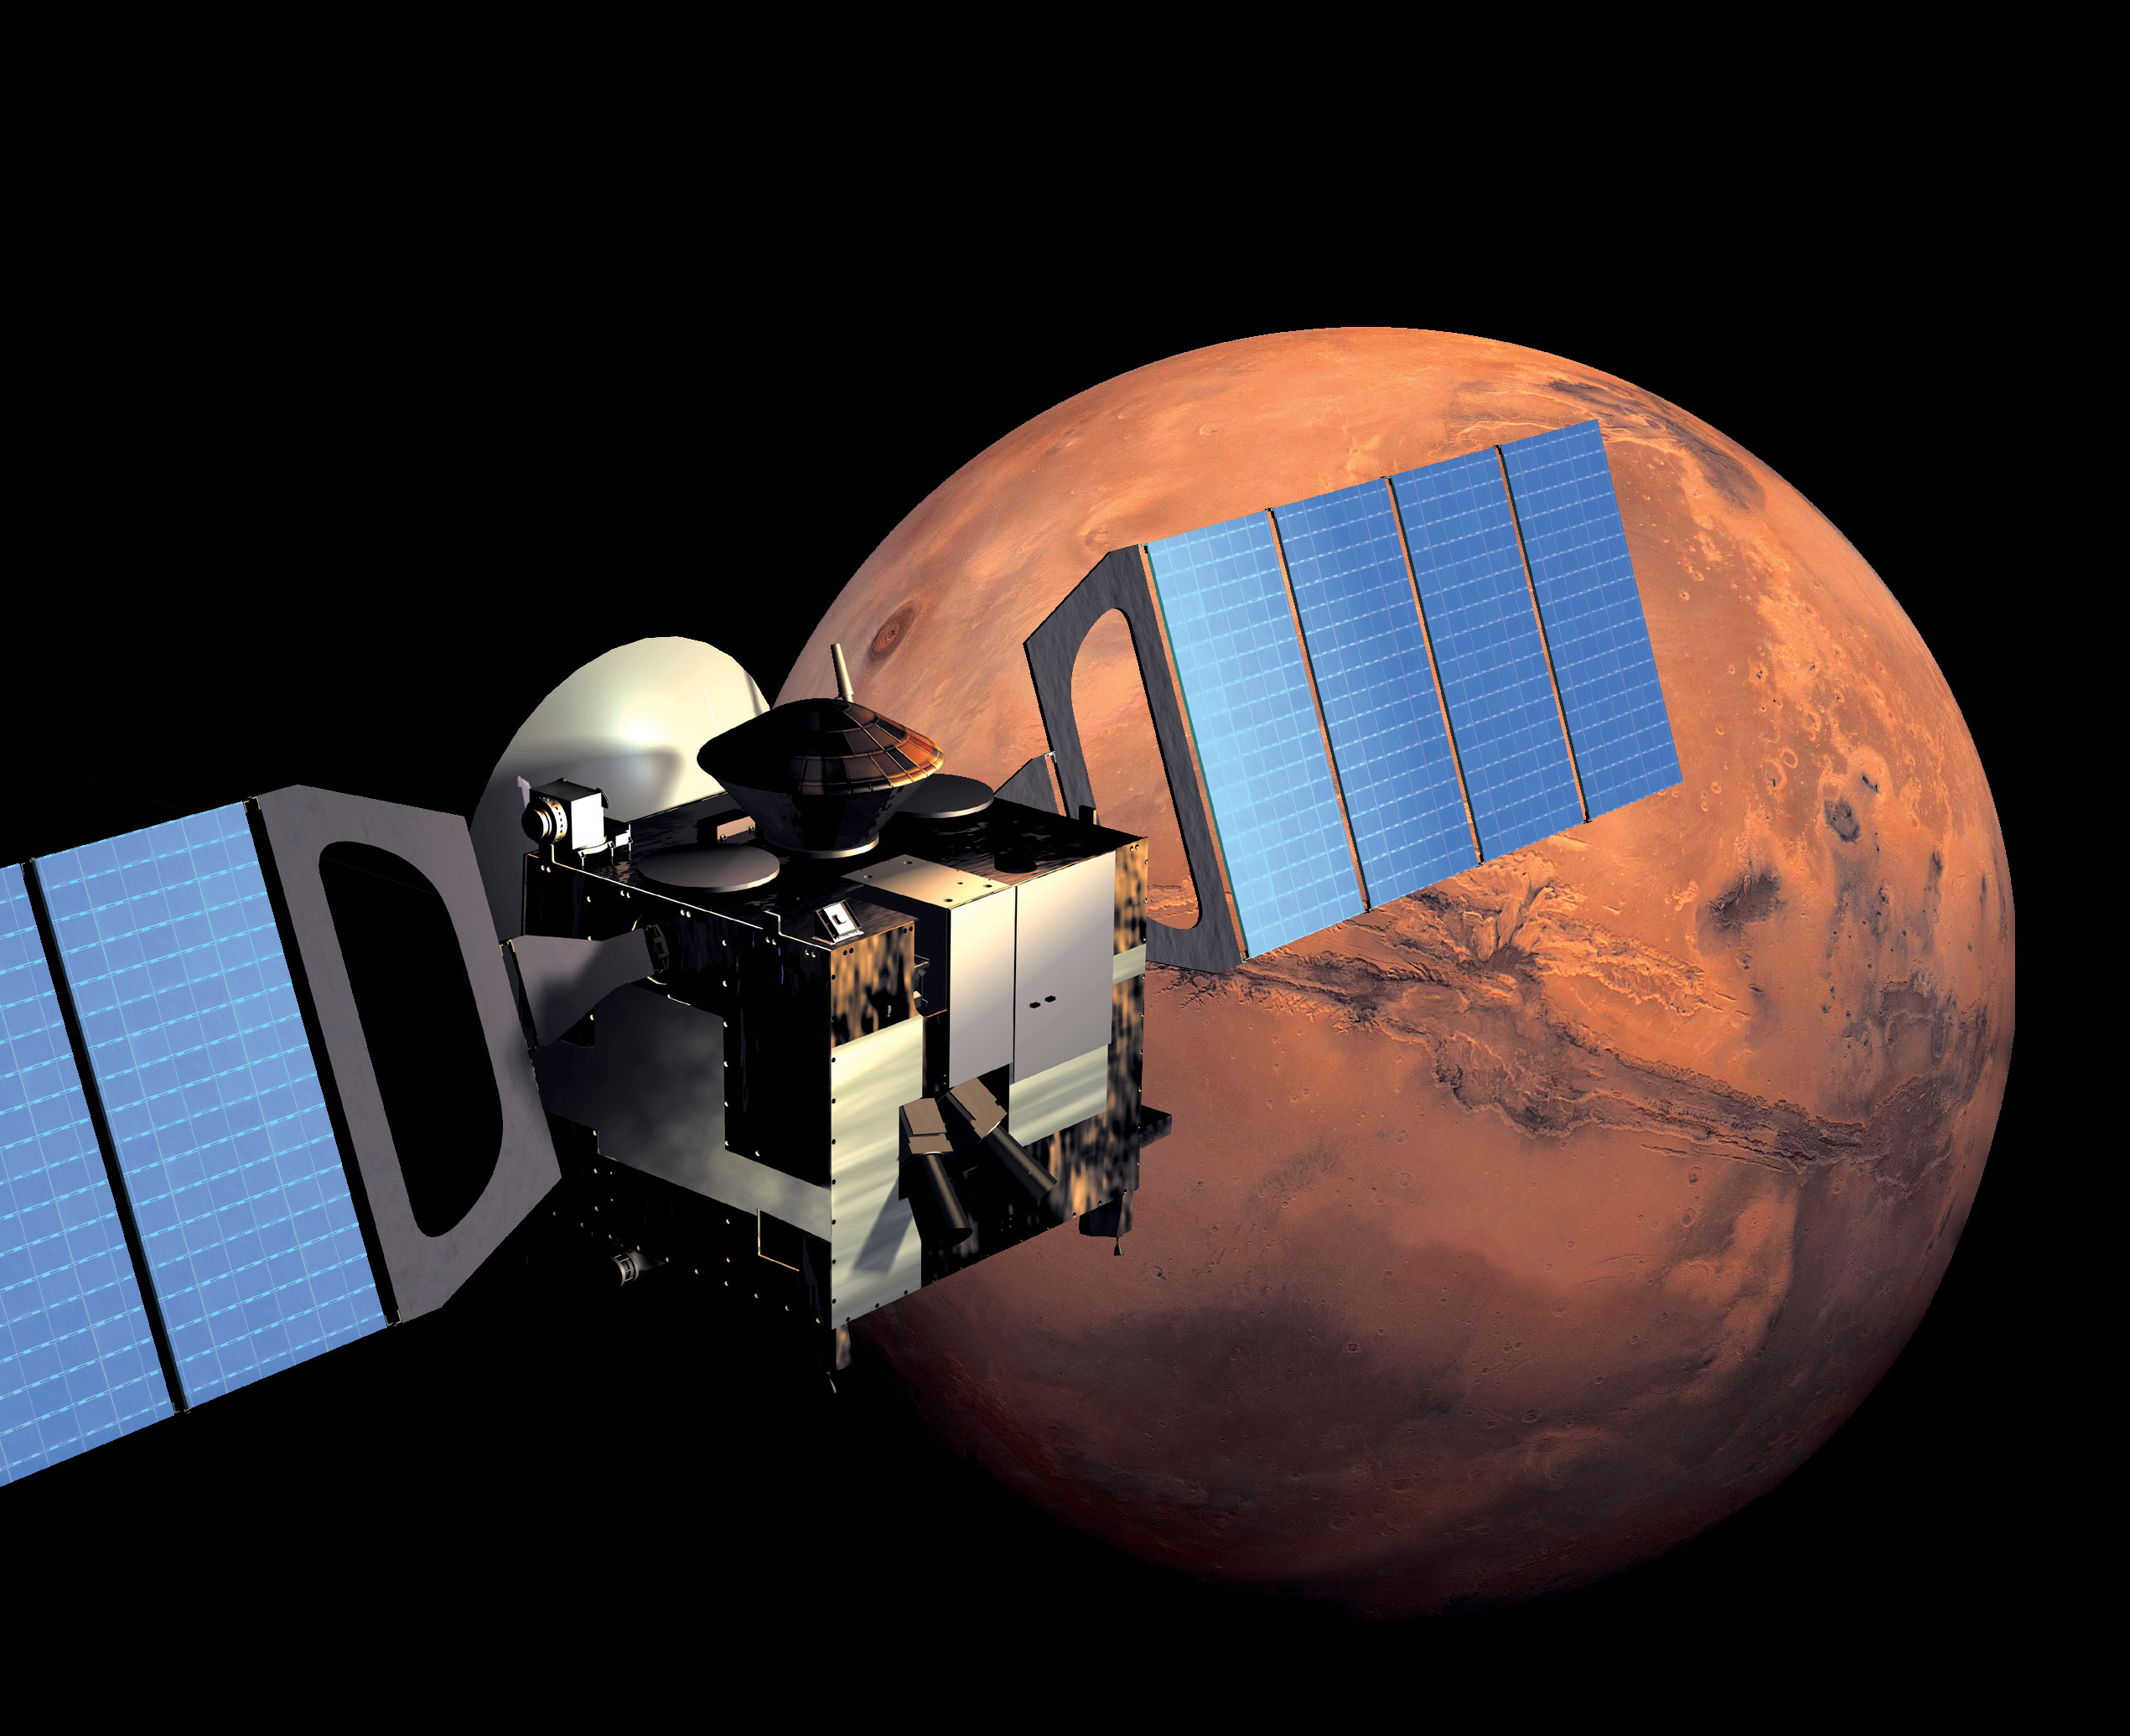
\includegraphics[width=140mm]{images/Mars.jpg}
	\caption{Mars Express spacecraft. Credit: ESA \citep{ESA2010}}
	\label{fig:mex}
\end{figure}

Why water? There is lots of geological evidence of former water occurrence. But before the~MEX~mission nobody had proved or refuted presence of water on~Mars in the present. Knowing more about water on Mars and its history, the scientists could postulate better hypotheses about the possibility of (former) life on the~planet \citep[p.~ix]{Chicarro2004}. \pdfcomment{Tady si nejsem uplne jisty tim, jak uvadet citace, protoze prakticky cela podkapitola cerpa z jedine knizky}

The original mission lifetime of MEX was projected up~to the~end of~2005 (which would be 1~Martian~year = 687~Earth~days) \citep{ESA2004}. However, overcoming some small problems (as the Solid State Mass Memory anomalies described in~\citep{ESA2011} or the~MARSIS~antennas deployment problems in~2004~\citep{ESA2004a,ESA2005}), MEX has worked on its science goals up to this day and its science mission was extended until~2014~\citep{ESA2013} (after 3~preceding extensions). Fred Jansen, MEX mission manager, said MEX had enough fuel for another 14~years of~operation (at the~beginning of~2012)~\citep{Clark2012}. So there is a hopeful prospect of further and deeper Mars exploration (eg. \citep{Gurnett2005}~discovered an~unexpected way of~using the MARSIS~instrument so that they ``added magnetometer functionality'' to~MARSIS).

\subsection{HRSC (\textit{High-Resolution Stereo Camera})}
HRSC is a high-resolution camera

\subsection{OMEGA (\textit{IR Mineralogical Mapping Spectrometer})}

\subsection{MARSIS (\textit{Mars Advanced Radar for Subsurface and Ionosphere
Sounding})}
